\documentclass{article}
\let\tldocenglish=1  % for live4ht.cfg
\usepackage{tex-live-zh-cn, indentfirst}
\usepackage{graphicx}
\usepackage{color}
\usepackage{xcolor}
\usepackage{verbatim}
\usepackage{comment}
\usepackage{minted}
\definecolor{bg}{rgb}{0.95,0.95,0.95}

\begin{document}

\title{%
  {\huge \textsf{Ganglia}\\\smallskip}%
  {\small \textit{搭建和介绍使用方法}}
}

\author{
        \email{quqinglei@icloud.com} 
       }

\maketitle
\begin{multicols}{2}
\tableofcontents
\end{multicols}

\section{Ganglia 介绍}
\subsection{简介}
Ganglia是UC Berkeley发起的一个开源集群监视项目,设计用于测量数以千计的节点。Ganglia的核心包含gmond、gmetad以
及一个Web前端。主要是用来监控系统性能,如:cpu 、mem、硬盘利用率, I/O负载、网络流量情况等,通过曲线很容易见
到每个节点的工作状态,对合理调整、分配系统资源,提高系统整体性能起到重要作用。

每台计算机都运行一个收集和发送度量数据的名为 gmond 的守护进程。接收所有度量数据的主机可以显示这些数据并且可以
将这些数据的精简表单传递到层次结构中。正因为有这种层次结构模式,才使得 Ganglia 可以实现良好的扩展。gmond 带来
的系统负载非常少,这使得它成为在集群中各台计算机上运行的一段代码,而不会影响用户性能。所有这些数据多次收集会
影响节点性能。网络中的 "抖动" 发生在大量小消息同时出现时,可以通过将节点时钟保持一致,来避免这个问题。

gmetad可以部署在集群内任一台节点或者通过网络连接到集群的独立主机,它通过单播路由的方式与gmond通信,收集区域内
节点的状态信息,并以XML数据的形式,保存在数据库中。

由RRDTool工具处理数据,并生成相应的的图形显示,以Web方式直观的提供给客户端。

官网地址:\url{http://ganglia.sourceforge.net/}

\subsection{工作原理}
Ganglia包括如下几个程序,他们之间通过XDL(xml的压缩格式)或者XML格式传递监控数据,达到监控效果。集群内的节点 ,
通过运行gmond收集发布节点状态信息,然后gmetad周期性的轮询gmond收集到的信息,然后存入rrd数据库,通过web服务
器可以对其进行查询展示。

\begin{figure}[H]
\centering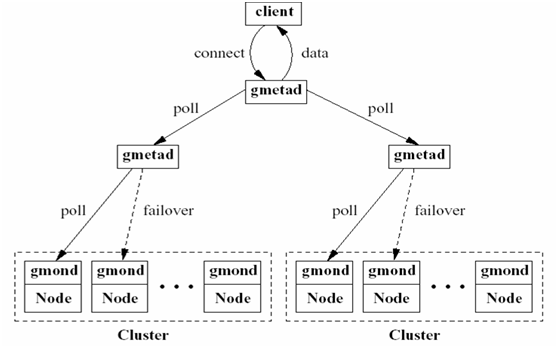
\includegraphics[width=6in]{pics/01.png}
\caption{工作原理}\label{fig:1}
\end{figure}

\section{安装}
我们刚才提到过ganglia 是由gmond、gmetad以及gweb三部分组成的,安装较为简单,这三部分分别安装完后稍微配置一下
就可以了,步骤如下:

\subsection{gmond}
gmond 意思是Ganglia的监控守护进程。它是一个轻量级服务,必须安装在每一个你需要采集数据的节点机上。

\textbf{安装依赖}
gmond 安装方法很简单,在现代Linux发行版上基本都有它需要的动态库,它需要libconfuse,pkgconfig,PCRE,APR 库。
在大多数发行版上都有其安装包,所以如果你使用包管理的Linux发行版解决依赖关系就不需要你操心了,简单的运行
包管理工具自动安装就可以了。下面是不同发行版的安装方式。

\begin{minted}[linenos, frame=lines, framesep=2mm]{sh}
# 基于 debian 的发行版,debian 基本都拥有此包
user@host:# apt-get install ganglia-monitor

# 基于 RPM 管理的发行版
user@host:# yum search ganglia-gmond

# 如果查不到可以使用一下命令添加软件仓库

# Red Hat 5.x:
user@host:# rpm -Uvh \ # 32 bit
http://mirror.ancl.hawaii.edu/linux/epel/5/i386/epel-release-5-4.noarch.rpm

user@host:# rpm -Uvh \ # 64 bit
http://mirror.ancl.hawaii.edu/linux/epel/5/x86_64/epel-release-5-4.noarch.rpm

# Red Hat 6.x
user@host:# rpm -Uvh \ # 32 bit
http://mirror.ancl.hawaii.edu/linux/epel/6/i386/epel-release-5-4.noarch.rpm

user@host:# rpm -Uvh \ # 64 bit
http://mirror.ancl.hawaii.edu/linux/epel/6/x86_64/epel-release-5-4.noarch.rpm

user@host:# yum install ganglia-gmond

# 如果没法通过网络安装,可以采用编译的方式,去官网下载源代码编译安装
\end{minted}

\subsection{gmetad}
gmetad 从其他gmetad或者gmond获取数据,并存储数据到rrd格式的文件。它提供了一个简单的查询组用于搜集特定信息
的机制,并支持分级授权,使人们可以建立联合监控域。

\textbf{安装依赖}
安装依赖了gmond基本一样,但需要安装RRDtool,用来存放数据,使用包管理工具,可自动处理此依赖

\begin{minted}[linenos, frame=lines, framesep=2mm]{sh}
# 基于 debian 的发行版,debian 基本都拥有此包
user@host:# apt-get install gmetad

# 基于 RPM 管理的发行版
user@host:# yum install ganglia-gmetad
\end{minted}

\subsection{gweb}
Ganglia 需要gweb才能完整,它提供一个PHP为前端的UI。

\textbf{安装依赖}
Ganglia 3.4.0 以后,前端就被分离出来了,且版本号和gmond以及gmetd都不再一致。gweb 3.4.0 支持所有版本的
gmond/gmetad 3.1.x 或者更高版本。具体还是看官方文档怎么写的,下面是依赖:

\begin{itemize}
\item Apache Web Server
\item PHP 5.2 or later
\item PHP JSON extension installed and enabled
\end{itemize}

\begin{minted}[linenos, frame=lines, framesep=2mm]{sh}
# 基于 debian 的发行版,debian 基本都拥有此包
user@host:# apt-get install apache2 php5 php5-json

# 测试配置文件中是否启用了 json 模块
user@host:#  grep ^extension=json.so /etc/php5/conf.d/json.ini
# 如果json模块没有启用,可以通过以下步骤
user@host:# echo 'extension=json.so' >> /etc/php5/conf.d/json.ini

# 执行完以上步骤,可以去官网下载gweb包,解压到 /var/www/ 路径,并重命名为 ganglia
root@host:# tar -xzvf ganglia-web-major.minor.release.tar.gz 
root@host:# mv ganglia-web-major.minor.release ganglia
root@host:# cd ganglia
root@host:# make install
root@host:# cd /var/www
root@host:# chown -R www-data:www-data ganglia

# 以上步骤就安装好了,重启apache2 服务器,就能在http://localhost/ganglia 里面看到页面了

# 基于 RPM 管理的发行版
user@host:# yum install httpd php

# 接下来安装PHP5.2 并配置好JSON的支持,这个和debian差不多,具体问题具体分析吧,下面基本就一样了
# 注意 chown 的时候应该把权限赋给apache用户,查看/etc/passwd 文件看看,应该是apache


# 注:在基于debian的系统上可以直接使用包管理工具安装WEB端
user@host:# apt-get install ganglia-webfrontend
user@host:# mv /usr/share/ganglia-webfrontend/ /var/www/ganglia
user@host:# chown -R www-data:www-data /var/www/ganglia
\end{minted}

\section{模块}
ganglia 支持添加模块,并支持添加C、Python、Perl、bash 的数据采集模块,可以理解成插件,它使用了Apache 的apr 来
加载。具体编写方法每种语言是不同的,但我们使用的绝大部分插件它已经提供了,所以基本上不需要我们再另行编写,关于
如何编写的具体方式可以查看:\url{http://sourceforge.net/apps/trac/ganglia/wiki/} 在这里就不做过多的介绍了。

\section{配置}
\subsection{gmond}
\textbf{配置文件名:\dirname{gmond.conf}} 

该文件一般位于\dirname{/etc/ganglia/gmond.conf} 路径。

\textbf{描述}

此文件为gmond所使用,是此守护进程的配置文件,包含要收集数据的一些配置,下面具体讲解一下:

\textbf{具体配置讲解}

\begin{itemize}
\item 配置中的配置项是大小写敏感的
\item 有些节的配置是可以重复,有些不可以,你只能设置一个 \code{cluster} 但可以设置很多的\code{module}
\end{itemize}

\textbf{cluster}

此配置文件中的cluster项只能配置一个,这个配置控制着UI上的报告,即此机器属于哪个集群。它有四个属性:name, owner,
latlong, url.

\begin{minted}[linenos, frame=lines, framesep=2mm]{sh}
 cluster {
    name = "Millennium Cluster"
    owner = "UC Berkeley CS Dept."
    latlong = "N37.37 W122.23"
    url = "http://www.millennium.berkeley.edu/";
  }
\end{minted}

\begin{description}
\item[name] 定义集群名称,也就是此台机器属于哪个集群
\item[owner] 集群管理者的名字,name和owner在所有集群中必须唯一
\item[latlong] GPS经纬度,即机器的地理位置,当然可以不写,根据自己的情况来啦
\item[url] 集群的信息,具体查询位置,当然可以不写,必经不是每个集群都有网站说明
\end{description}

\textbf{host}

\begin{minted}[linenos, frame=lines, framesep=2mm]{sh}
 host {
   location = "1,2,3"
 }
\end{minted}

机架位子,根据自己的情况来,可以不写

\textbf{globals}

\begin{minted}[linenos, frame=lines, framesep=2mm]{sh}
 globals {
    daemonize = true
    setuid = true
    user = nobody
    host_dmax = 3600
  }
\end{minted}

\begin{description}
\item[daemonize] 是否以守护进程的形式启动,一般设为true
\item[setuid] 为真时,将设置其有效的有用户指定的uid,为假时不会改变他的有效用户,默认为真
\item[user] 这个和上面的一项有关系,即这个进程以哪个用户启动,如果使用包管理工具,它的默认值应该是ganglia
当然可以是其他用户,一般来说在Linux下为了安全会把软件安装到不同的用户下,这样权限划比较合理。
\item[host\_dmax] 这个一般设置为0,它的单位是秒,如果设置了数,当此机器在此时间内不再报告,gmond会删除它
\end{description}

\textbf{udp\_send\_channel}

可以把它理解成为转发,gmond可以转发数据到其他gmond上,这样在收集数据的时候只需要读取那一个gmond上的数据。

\begin{minted}[linenos, frame=lines, framesep=2mm]{sh}
 udp_recv_channel {
    port = 8666
    family = inet4
  }
  udp_recv_channel {
    port = 8666
    family = inet6
  }
\end{minted}

\textbf{udp\_recv\_channel}

\textbf{tcp\_accept\_channel}

以上三个功能分别为转发、接收、TCP协议,具体使用功能待测,没有完全理解[tbd]

\textbf{collection\_group}
这项可以设置很多,使用\code{gmond -m} 能得到所有的内置测量工具,格式如下:
\begin{minted}[linenos, frame=lines, framesep=2mm]{sh}
collection_group {
    collect_once   = yes
    time_threshold = 1800
    metric {
     name = "cpu_num"
     title = "Number of CPUs"
    }
  }

 collection_group {
    collect_every = 60
    time_threshold = 300
    metric {
      name = "cpu_user"
      value_threshold = 5.0
      title = "CPU User"
    }
    metric {
      name = "cpu_idle"
      value_threshold = 10.0
      title = "CPU Idle"
    }
  }
\end{minted}

\begin{description}
\item[collect\_once] 上面的意思是在重启之前只搜集一次信息
\item[time\_threshold] 上面的1800代表1800秒发送一次cpu\_num 的数据
\item[name] 内置的采集器名称,可以通过\code{gmond -m} 获得所有的内置数据采集器
\item[title] 这个可以根据情况设了,就是一个描述字段
\item[collect\_every] 数据采集间隔时间,单位为秒
\end{description}

\textbf{modules}

这个是插件的配置信息,ganglia支持插件,也就是非内置的信息采集方式,用户可以根据它提供的格式写一些
插件,基本上不用写了,在其官网上有我们能用到的几乎所有插件。

\begin{minted}[linenos, frame=lines, framesep=2mm]{sh}
modules {
     module {
       name = "example_module"
       enabled = yes
       path = "modexample.so"
       params = "An extra raw parameter"
       param RandomMax {
         value = 75
       }
       param ConstantValue {
         value = 25
       }
     }
   }

modules { 
  module { 
    name = "core_metrics" 
  }   
  module { 
    name = "cpu_module" 
    path = "/usr/lib/ganglia/modcpu.so" 
  }   
  module { 
    name = "disk_module" 
    path = "/usr/lib/ganglia/moddisk.so" 
  }   
  module { 
    name = "load_module" 
    path = "/usr/lib/ganglia/modload.so" 
  }   
  module { 
    name = "mem_module" 
    path = "/usr/lib/ganglia/modmem.so" 
  }   
  module { 
    name = "net_module" 
    path = "/usr/lib/ganglia/modnet.so" 
  }   
  module { 
    name = "proc_module" 
    path = "/usr/lib/ganglia/modproc.so" 
  }   
  module { 
    name = "sys_module" 
    path = "/usr/lib/ganglia/modsys.so" 
  }   
} 
\end{minted}

\begin{description}
\item[name] 模块名,或者说插件名称
\item[path] 模块位置,上面的例子主要是动态链接库,其实它还支持其他语言编写的插件
\end{description}

\textbf{include}

配置文件可以再包含其他配置文件,这个基本上是为了扩展其他语言而定义的此项

\begin{minted}[linenos, frame=lines, framesep=2mm]{sh}
include ('/etc/ganglia/conf.d/*.conf')
\end{minted}

\textbf{access control}

访问控制

\begin{minted}[linenos, frame=lines, framesep=2mm]{sh}
acl {
    default = "deny"
    access {
      ip = 192.168.0.4
      mask = 32
      action = "allow"
    }
  }
\end{minted}

udp\_recv\_channel 和 tcp\_accept\_channel 可以设置访问控制列表,第一个例子会拒绝来自192.168.0.4的数据包
第二个例子默认允许接收来自192.168.0.0 子网的所有数据包

\section{备注}
ganglia 的配置方式比较简单,可以采用其作为hadoop的集群监控软件和测试Hadoop性能的工具,或者其他集群的监控
工具,也可以配合nagios。在思考是否可以从中提取一些有效信息为Hadoop混合型集群的任务分配提供数据依据。

\end{document}
